\documentclass[a4paper,12pt]{book}
\usepackage[utf8]{inputenc}
\title{}
\author{Rachel Morris}
\date{\today}

\usepackage{rachwidgets}
\usepackage{fancyhdr}
\usepackage{lastpage}
\usepackage{boxedminipage}

\pagestyle{fancy}
\fancyhf{}
\lhead{CS 250}
\chead{Fall 2017}
\rhead{Lab 1: STL Containers}
\rfoot{\thepage\ of \pageref{LastPage}}
\lfoot{By Rachel Morris, last updated \today}

\graphicspath{ {images/} }

\renewcommand{\headrulewidth}{2pt}
\renewcommand{\footrulewidth}{1pt}

\begin{document}

    \chapter*{Lab 1: STL Containers} \stepcounter{chapter}
        \section*{Information}
            \paragraph{ Topics: } vector, list, stack, queue, map
            \paragraph{ Turn in: } All .cpp files, question document as .txt file. \\
                \tab[2.3cm] Every lab \textit{ part } should have its own .cpp file. \\
                \tab[2.3cm] Give each lab file a unique name, like \texttt{ lab1\_part1.cpp }.

            \paragraph{ Penalties: }
                The following items will negatively impact your score.

                \begin{itemize}
                    \item   \textbf{Program doesn't build}
                        \\ Your program should always build. Programs turned in that don't build will automatically receive a grade of 50\%.{}
                            Additionally, I build your code from the command line in Linux; Your code should be portable. Certain features
                            are allowed in Visual Studio or Windows but don't work for all compilers. \\
                            \footnotesize Avoid: \texttt{\#pragma once}, \texttt{system("pause");}, ignoring filename cases
                            \normalsize 
                    \item   \textbf{Missing source files}
                        \\ If your .hpp or .cpp files are missing, they cannot be graded and will result in a 0\%. Always double-check to make sure you're submitting all your files.
                    \item   \textbf{Visual Studio files}
                        \\ I don't want these. I ONLY want your .hpp and .cpp files. I won't count off if you turn it in, but do me a favor (and help me grade quickly) by not turning in junk files.
                    \item   \textbf{Zipped files}
                        \\ I don't want this. Just submit your source files. I won't count off if you turn in a zip, but when I download assignments they're already zipped so it just makes more work for me.
                \end{itemize}

% ----------------------------------------------------------------------
% ----------------------------------------------------------------------
% ----------------------------------------------------------------------
            \subsection*{Part 1: STL Vector}
            
                \begin{intro}{STL Vector functions}

                    \footnotesize
                    
                    \texttt{ void vector::push\_back( value\_type\&  value ) }

                        Adds a new element at the end of the vector, after its current last element.
                        The content of val is copied (or moved) to the new element. \\
                    
                    \texttt{ unsigned int vector::size() }

                        Returns the number of elements in the vector. \\
                    
                    \texttt{ value\_type\& vector::operator[]( size\_type n ) }

                        Returns a reference to the element at position n in the vector container. \\
                    
                    

                    \raggedleft{ \tiny{ http://www.cplusplus.com/reference/vector/vector/ }}
                    
                \end{intro}
            
                We will start out by working with the \textbf{ vector } object
                of the Standard Template Library.  You can view the documentation
                for this object at
\begin{verbatim}
http://www.cplusplus.com/reference/vector/vector/ 
\end{verbatim}
                \hrulefill{}
                \subsubsection*{ Starter code }
                    Begin with the following code:

% code box %
\begin{lstlisting}[style=code]
#include <iostream> // required for cout
#include <vector>   // required for vector
#include <string>   // required for strings
using namespace std;

void AddIngredients( vector<string>& ingredients )
{
}

void DisplayIngredients( const vector<string>& ingredients )
{
}

int main()
{ 
    return 0;
}
\end{lstlisting}
% code box %

                    ~\\
                    Notice that the functions \texttt{ AddIngredients(...) }
                    and \texttt{ DisplayIngredients(...) } both contain
                    \texttt{ vector } parameters. Vectors are essentially
                    like \textit{ dynamic arrays }, and they can store any
                    data type. In this case - these vectors will store
                    \texttt{ strings }.

                    The \texttt{ AddIngredients(...) } function will be responsible
                    for inserting new strings into the vector, so the
                    vector parameter is being passed in \textbf{ by-reference },
                    denoted by the \&.

                    The \texttt{ DisplayIngredients(...) } function will only
                    display the values stored in the vector, so the parameter
                    is passed as a \textbf{ const reference }. Why?
                    -- Because a vector could be a large object, so it is
                    more efficient to pass it by-reference than by-value.
                    Passing by-value means copying all the data, and that could
                    be \textit{ computationally expensive }.

                \hrulefill{}
                \subsubsection*{ main() }
    
                    Within \texttt{ main() }, create a
                    \texttt{ vector } of
                    \texttt{ strings } named
                    \textbf{ ingredients }

\begin{verbatim}
    vector<string> ingredients;
\end{verbatim}

                    ~\\ Next, \textit{ call } the \texttt{ AddIngredients(...) }
                    function, passing in the \textbf{ ingredients } variable
                    as the argument.
\begin{verbatim}
    AddIngredients( ingredients );
\end{verbatim}

                    ~\\ Finally, \textit{ call } the \texttt{ DisplayIngredients(...) }
                    function, again passing in the \textbf{ ingredients } variable
                    as the argument. 
\begin{verbatim}
    DisplayIngredients( ingredients );
\end{verbatim}

                    ~\\
                    Now the vector variable is being passed around, but
                    these functions currently don't do anything. We will
                    implement these next.

                    % Intro
                    \begin{intro}{ Review: Parameter vs. Argument }

                    When you're writing a function, the
                    variables declared within the ( ) are
                    called \textbf{ parameters }. \\

                    When you're passing data \textit{ into }
                    a function call, the items that you're passing in are
                    called \textbf{ arguments }.

                    When passing arguments, you can use variables
                    or literals. When passing in a variable, you
                    do not need to specify its data type. \\

                    When a parameter is \textbf{ pass-by-reference },
                    then you can only pass in a variable. No special
                    symbols are required from the argument side. 
                    \end{intro}


                \hrulefill{}
                \subsubsection*{ void AddIngredients( vector$<$string$>$\& ingredients ) }

                    The \texttt{ vector } class has a function called
                    \texttt{ push\_back }, which allows us to add a
                    new item to the back of the vector's internal array.
                    You can read the documentation for \texttt{ push\_back } at
\begin{verbatim}
    http://www.cplusplus.com/reference/vector/vector/push_back/    
\end{verbatim}

                    The \texttt{ push\_back } function has a \texttt{ void }
                    return type, and its only parameter is a new value.
                    The data type of the parameter depends on what the
                    vector has been declared with. In our case, it is a
                    \texttt{ string }.

                    Using the \texttt{ push\_back } function, insert the
                    following items into the vector: (1) lettuce,
                    (2) tomato, (3) mayo, and (4) bread.

\begin{verbatim}
    ingredients.push_back( "lettuce" );
\end{verbatim}

                \hrulefill{}
                \subsubsection*{ void DisplayIngredients( const vector$<$string$>$\& ingredients ) }
                    The \texttt{ vector } class has a function \texttt{ size() }
                    that will return an \texttt{ unsigned integer } with
                    the count of items in the vector.

                    You can also access items at specific elements of the
                    array with the \textbf{ subscript operator },
                    $ [ $ $ ] $. The vector uses an array behind-the-scenes,
                    so you can access the first element at position 0, like:
                    \texttt{ ingredients $[$ 0 $]$ } ~\\


                    \begin{hint}{ Hint: Iterating over an array }
                       Maybe you're feeling a little rusty. For an array of size $ n $,
                       how do we iterate over all its elements to display them?

\begin{verbatim}
    for ( int i = 0; i < n; i++ )
    {
        cout << i << ". " << arr[i] << endl;
    }
\end{verbatim}

                        Make sure you review your \textbf{ core C++ contepts }
                        so that you can spend more time on the design of the
                        data structures in this course, instead of struggling
                        with how to write the basics.
                    \end{hint}

                    Use a \texttt{ for loop } to iterate over all items
                    in the vector \\ ( index $ 0 $ to $ size - 1 $ ), and display
                    both the index of each vector element, and its value,
                    using a \texttt{ cout } statement.

                    Your program output should look like the following.
% program output %
\begin{lstlisting}[style=output]
0. lettuce
1. tomato
2. mayo
3. bread
\end{lstlisting}
% program output %


            \newpage
            % Intro
            \begin{intro}{ Review: Arrays }

            Recall from previous programming courses that
            when you create an array in C++, the elements
            of the array are stored \textbf{ side-by-side }
            in memory. This is the reason that we can
            \textbf{ randomly access } elements of the array,
            because if we know the address of the first element,
            then we simply need to step to an offset of
            $ index \times bytes $ to find the element at that index. \\

            \texttt{ int arr[3] = } ~\\

            \begin{center}
                \begin{tabular}{ | c | c | }
                    \hline
                    \textbf{ index } & \textbf{ address } \\ \hline

                    0 & \texttt{ 0x7ffee961a920 }
                    \\ \hline

                    1 & \texttt{ 0x7ffee961a924 }
                    \\ \hline

                    2 & \texttt{ 0x7ffee961a928 }
                    \\ \hline
                    
                \end{tabular}
            \end{center}
            
            ~\\ The size of an integer is 4 bytes, so notice the addresses of the elements are different by 4.
            \texttt{ 0x...20, \tab 0x...24, \tab 0x...28 }
            
            \end{intro}
            % End intro 

            \hrulefill{}
            \newpage
% ----------------------------------------------------------------------
% ----------------------------------------------------------------------
% ----------------------------------------------------------------------
            \subsection*{Part 2: STL List}

                \begin{intro}{STL List functions}

                    \footnotesize
                    
                    \texttt{ void list::push\_back( value\_type\&  value ) }

                        Adds a new element at the end of the list container, after its current last element.
                        The content of val is copied (or moved) to the new element. \\
                    
                    \texttt{ void list::push\_front( value\_type\&  value ) }

                        Inserts a new element at the beginning of the list, right before its current first element.
                        The content of val is copied (or moved) to the inserted element. \\
                    
                    \texttt{ void list::sort() }

                        Sorts the elements in the list, altering their position within the container. \\
                    
                    \texttt{ void list::reverse() }

                        Reverses the order of the elements in the list container. \\
                    

                    \raggedleft{ \tiny{ http://www.cplusplus.com/reference/list/list/ }}
                    
                \end{intro}




            
                The \textbf{ list } is another type of linear data
                structure from the Standard Template Library. Unlike
                the \texttt{ vector }, however, the List is not implemented
                with an array, but a series of ``nodes'' that point at the
                next element in the list. Because of this, you cannot
                \textbf{ randomly access elements } of a list like you can
                with a vector or an array.
\begin{verbatim}
http://www.cplusplus.com/reference/list/list/
\end{verbatim}

                \hrulefill{}
                \subsubsection*{ Starter code }
                    Begin with the following code:

% code box %
\begin{lstlisting}[style=code]
#include <iostream> // required for cout
#include <list>     // required for list
#include <string>   // required for strings
using namespace std;

void AddCourses( list<string>& courses )
{
}

void SortList( list<string>& courses )
{
}

void ReverseList( list<string>& courses )
{
}

void DisplayCourses( list<string>& courses )
{
    int counter = 0;
    // This is how we have to iterate thru a list.
    for( list<string>::iterator it = courses.begin();
        it != courses.end(); it++ )
    {
        if ( counter != 0 ) { cout << ", "; }
        cout << counter++ << ". " << (*it);
    }
}

int main()
{
    return 0;
}
\end{lstlisting}
% code box %

                \hrulefill{}
                \subsubsection*{ main() }
                    First, in \texttt{ main() }, create a new list
                    that will store strings, like this:

\begin{verbatim}
    list<string> courses;
\end{verbatim}

                    Then call \texttt{ AddCourses(...) }, passing in
                    the \texttt{ courses } variable as the argument.
                    Afterward, call \texttt{ DisplayCourses(...) }. \\

                    Next, call \texttt{ SortList(...) } and then
                    \texttt{ DisplayCourses(...) }. \\

                    And finally, call \texttt{ ReverseList(...) } and then
                    \texttt{ DisplayCourses(...) }. \\

                    \texttt{ DisplayCourses(...) } has already been
                    written for you because using a for loop on a
                    \texttt{ list } object requires using \texttt{ iterators };
                    we can't just iterate from $ i = 0 $ to $ size-1 $
                    like with a \texttt{ vector }.
                    
                \hrulefill{}
                \subsubsection*{ void AddCourses( list$<$string$>$\& courses ) }

                    With the \texttt{ list }, we can add new items to the
                    \textbf{ front }, using \texttt{ push\_front(...) }
                    or to the \textbf{ back }, using \texttt{ push\_back(...) }. \\

                    Add the following items to the \texttt{ courses } list,
                    at either the front or the back:
                    \textit{ cs 250, cs 200, cs 210, cs 235, cs 134, cs 211 }
                
                \hrulefill{}
                \subsubsection*{ void SortList( list$<$string$>$\& courses ) }
                    The \texttt{ list } class contains a function called
                    \texttt{ sort() } that will sort all the elements in
                    the list for you. Call it from this function.

                \hrulefill{}
                \subsubsection*{ void ReverseList( list$<$string$>$\& courses ) }
                    The \texttt{ list } class contains a function called
                    \texttt{ reverse() } that will reverse the order of
                    elements in the list. Call it with this function.


                \hrulefill{}
                
                
                ~\\ Running the program, your output will look something like...
% program output %
\begin{lstlisting}[style=output]
Normal order
0. cs 250, 1. cs 200, 2. cs 235, 3. cs 210, 4. cs 134, 5. cs 211

Sorted order
0. cs 134, 1. cs 200, 2. cs 210, 3. cs 211, 4. cs 235, 5. cs 250

Reverse order
0. cs 250, 1. cs 235, 2. cs 211, 3. cs 210, 4. cs 200, 5. cs 134
\end{lstlisting}
% program output %
                    (Note: The first output will look different based on
                    the order you put the items in.)


                
            % Intro
            \begin{intro}{ Linked Lists }

            Later in the class, we will be working with \textbf{ linked lists }.

            Linked lists use \textbf{ pointers } to create nodes for a list,
            by allocating memory for new nodes as needed...

    \footnotesize 
\begin{verbatim}

    Node* newNode = new Node();
    newNode->data = 123;
    
    newNode->ptrPrevious = ptrLast; // Link them together
    ptrLast->ptrNext = newNode;

    ptrLast = newNode // Update the address ptrLast is pointing to
\end{verbatim}

            The \textbf{ STL List } is implemented with a \textbf{ doubly-linked list }

            
            \end{intro}
            % End intro 

                \begin{figure}[h]
                    \centering
                    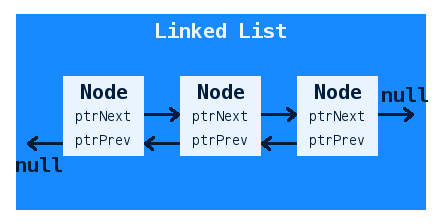
\includegraphics[height=3.5cm]{lab01-basic-linked-list}
                \end{figure}









                    

            \newpage
% ----------------------------------------------------------------------
% ----------------------------------------------------------------------
% ----------------------------------------------------------------------
            \subsection*{Part 3: STL Queue}

                \begin{intro}{STL Queue functions}

                    \footnotesize
                    
                    \texttt{ value\_type\& queue::front() }

                        Returns a reference to the next element in the queue.
                        The next element is the "oldest" element in the queue and the
                        same element that is popped out from the queue when queue::pop is called. \\
                    
                    \texttt{ void queue::push( const value\_type\& val ) }

                        Inserts a new element at the end of the queue, after its current last element.
                        The content of this new element is initialized to val. \\

                    
                    \texttt{ void queue::pop() }

                        Removes the next element in the queue, effectively reducing its size by one.
                        The element removed is the "oldest" element in the queue whose value can be
                        retrieved by calling member queue::front. \\
                    
                    \texttt{ bool queue::empty() }

                        Returns whether the queue is empty: i.e. whether its size is zero. \\

                    \raggedleft{ \tiny{ http://www.cplusplus.com/reference/queue/queue/ }}
                    
                \end{intro}

            
                A \textbf{ queue } is a type of data structure that
                is linear in nature, but access to the elements are
                restricted. Queues can be implemented with arrays or
                with list structures. ~\\

                
                \begin{figure}[h]
                    \centering
                    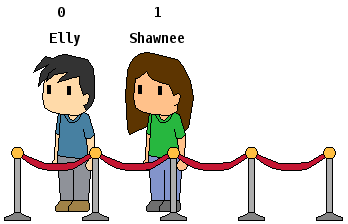
\includegraphics[height=4cm]{lab01-queue-a}
                \end{figure}

                \newpage
                ~\\ Items can be \textbf{ pushed } into the back of the queue,
                just as if you were lining up at the store. ~\\

                \begin{figure}[h]
                    \centering
                    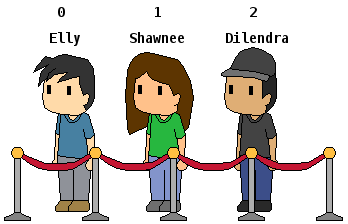
\includegraphics[height=4cm]{lab01-queue-b}
                \end{figure}

                ~\\ The first item that gets to leave the queue is the item at the \textbf{ front. }
                Then, everything gets moved forward one spot.
                ~\\

                \begin{figure}[h]
                    \centering
                    
\includegraphics[height=4cm]{lab01-queue-c}
                \end{figure}

                ~\\ We will be learning more about queues later
                in the semester, so it is good to get acquainted with them.

\begin{verbatim}
http://www.cplusplus.com/reference/queue/queue/
\end{verbatim}
                
                \hrulefill{}
                \subsubsection*{ Starter code }
                    Begin with the following code:

% code box %
\begin{lstlisting}[style=code]
#include <iostream> // required for cout
#include <string>   // required for strings
#include <queue>    // required for queues
using namespace std;

int main()
{
    float balance = 0.0;

    cout << "Final balance: $" << balance << endl;
    
    return 0;
}
\end{lstlisting}
% code box %

                \hrulefill{}
                \subsubsection*{ main() }

                    Within \texttt{ main() }, create a queue of \texttt{ floats }
                    called \textbf{ transactions }.

\begin{verbatim}
    queue<float> transactions;
\end{verbatim}

                    Create a series of values into the queue, both positive
                    and negative values. These will represent deposits and
                    withdraws into an account. The function to add an
                    item to the queue is \texttt{ push(...) }. \\

                    Create a while loop that will keep looping while
                    the queue is not empty. To check if the queue is
                    empty, use the \texttt{ empty() } function.
                    
                    While the queue is \textit{ not empty }...

                    \begin{itemize}
                        \item Access the front item in the queue with \texttt{ front() }.
                        Display this value with \texttt{ cout }, and also
                        add this value to the \texttt{ balance } variable.
                        \item Use the queue's \texttt{ pop() } function next
                        to remove the front item.
                    \end{itemize}

                    At the end of the program, the final balance will be displayed.

% program output %
\begin{lstlisting}[style=output]
100.42 pushed to account
-5.58 pushed to account
50.78 pushed to account
-20.50 pushed to account

Final balance: $125.12
\end{lstlisting}
% program output %
                    
            
            \newpage
% ----------------------------------------------------------------------
% ----------------------------------------------------------------------
% ----------------------------------------------------------------------
            \subsection*{Part 4: STL Stack}

                \begin{intro}{STL Stack functions}

                    \footnotesize
                    
                    \texttt{ value\_type\& stack::top() }

                        Returns a reference to the top element in the stack.
                        Since stacks are last-in first-out containers, the top
                        element is the last element inserted into the stack. \\
                    
                    \texttt{ void stack::push( const value\_type\& val ) }

                        Inserts a new element at the top of the stack,
                        above its current top element. The content of this
                        new element is initialized to a copy of val. \\

                    
                    \texttt{ void stack::pop() }

                        Removes the element on top of the stack, effectively reducing its size by one.
                        The element removed is the latest element inserted into the stack,
                        whose value can be retrieved by calling member stack::top. \\
                    
                    \texttt{ bool stack::empty() }

                        Returns whether the stack is empty: i.e. whether its size is zero. \\

                    \raggedleft{ \tiny{ http://www.cplusplus.com/reference/stack/stack/ }}
                    
                \end{intro}


            
                A \textbf{ stack } is similar to a queue in that
                access to its elements are also restricted,
                but what you can access is different.

                Stacks are usually visualized vertically, like a
                Pringles tube, where items being added fall to the bottom.
                Because of this, the first item added ends up being
                below all later items. ~\\

                \begin{figure}[h]
                    \centering
                    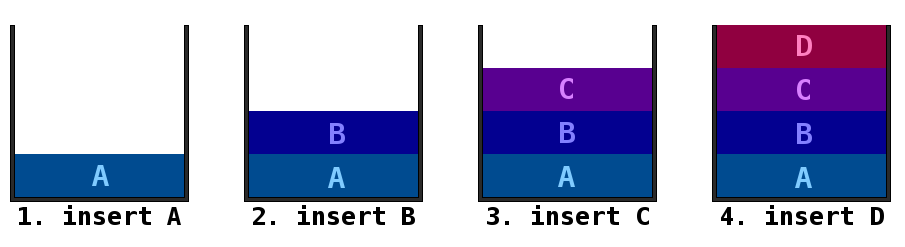
\includegraphics[height=4cm]{lab01-stacks.png}
                \end{figure}
                
                To add a new item to the stack, you use \texttt{ push(...) } 

                And to access the top-most item, you use \texttt{ top() }.
                
                To remove the top-most item, you use the \texttt{ pop() } function. 

                ~\\ View all of the stack's documentation at:
\begin{verbatim}
http://www.cplusplus.com/reference/stack/stack/
\end{verbatim}

                \hrulefill{}
                \subsubsection*{ Starter code }
                    Begin with the following code:

% code box %
\begin{lstlisting}[style=code]
#include <iostream>
#include <string>
#include <stack>
using namespace std;

int main()
{    
    bool done = false;

    cout << "Enter the next word of the sentence, or UNDO to undo, or DONE to stop." << endl;

    while ( !done )
    {
        string word;
        cout << ">> ";
        cin >> word;

        if ( word == "UNDO" )
        {
        }
        else if ( word == "DONE" )
        {
            done = true;
        }
        else
        {
        }
    }

    // Display stack of words
    cout << endl << endl << "Finished sentence: ";
    
    return 0;
}

\end{lstlisting}
% code box %

            
                \hrulefill{}
                \subsubsection*{ main() }

                    First in \texttt{ main() }, before the while loop starts,
                    create a stack of strings.
                    
\begin{verbatim}
    stack<float> sentence;
\end{verbatim}

                    As the user enters words, we will \textbf{ push } them
                    onto the sentence. \\

                    Within the \texttt{ if ( word == "UNDO" ) } statement,
                    display a message that you're removing the top-most item
                    from the stack, and then use the \texttt{ pop() } function
                    to remove the top-most item. \\

                    Within the \texttt{ else } statement,
                    use the \texttt{ push(...) } function to push the
                    \texttt{ word } onto the \texttt{ sentence } stack. \\

                    Finally, after the while loop has finished, create
                    a while loop that will \textit{ continue running while
                    the } \texttt{ sentence } \textit { stack is not empty. }
                    Within this loop:

                    \begin{itemize}
                        \item Display the top-most item with the \texttt{ top() } function.
                        \item Remove the top-most item with the \texttt{ pop() } function.
                    \end{itemize}

% program output %
\begin{lstlisting}[style=output]
Enter the next word of the sentence, or UNDO to undo, or DONE to stop.
>> up
>> you
>> let
>> UNDO
	 Removed let
>> give
>> gonna
>> never
>> DONE


Finished sentence: never gonna give you up 
\end{lstlisting}
% program output %

% program output %
\begin{lstlisting}[style=output]
Enter the next word of the sentence, or UNDO to undo, or DONE to stop.
>> a
>> b
>> c
>> UNDO
>> d
>> e
>> f
>> DONE


Finished sentence: f e d b a
\end{lstlisting}
% program output %
            
            \newpage
% ----------------------------------------------------------------------
% ----------------------------------------------------------------------
% ----------------------------------------------------------------------
            \subsection*{Part 5: STL Map}

                \begin{intro}{STL Map functions}

                    \footnotesize
                    
                    \texttt{ value\_type\& map::operator[]( const key\_type\& k ) }

                        If k matches the key of an element in the container,
                        the function returns a reference to its mapped value.
                        If k does not match the key of any element in the container,
                        the function inserts a new element with that key and returns a
                        reference to its mapped value. Notice that this always increases the container
                        size by one, even if no mapped value is assigned to the element
                        (the element is constructed using its default constructor).
                    

                    \raggedleft{ \tiny{ http://www.cplusplus.com/reference/map/map/ }}
                    
                \end{intro}

                    The \textbf{ map } type, sometimes known as a \textbf{ dictionary }
                    or \textbf{ hash-table }, is a type of data-structure that relates
                    some \textit{ key } to a \textit{ value }.

                    If we were looking at an average array, the keys would be
                    \texttt{ 0, 1, 2, 3, ... } and so on.
                    With a map, the key can be \textit{ any data-type },
                    and in \textit{ any order }. \\

                    For example, let's say we wanted to store an array of
                    employees, but rather than have employees 0, 1, 2, 3, etc.,
                    we want to be able to access employees directly via their
                    employee IDs, which are alphanumeric values. \\

                    \begin{center}
                        \begin{tabular}{ | l | l | }
                            \hline
                            \textbf{ key } & \textbf{ value }  \\ \hline
                                hr-32917 & Maryam A. \\ \hline
                                hr-38163 & Colton B. \\ \hline
                                eng-632 & Shelley C. \\ \hline
                                eng-192 & Logan D. \\ \hline
                                qa-291 & Elizabeth E. \\ \hline
                                qa-942 & Liangyan F. \\ \hline
                        \end{tabular}
                    \end{center}

                    Once stored in a map, we can access the values (the
                    employee names) via the key:
                    \texttt{ cout << employees[ "hr-32917" ] << endl; }
                    


                \hrulefill{}
                \subsubsection*{ Starter code }
                    Begin with the following code:

% code box %
\begin{lstlisting}[style=code]
#include <iostream>
#include <string>
#include <map>
using namespace std;

int main()
{
    while ( true )
    {
        string color;
        cout << endl << "Enter a color, or QUIT to stop: ";
        cin >> color;
        
        if ( color == "QUIT" )
        {
            break;
        }
    }
    
    return 0;
}
\end{lstlisting}
% code box %

                \hrulefill{}
                \subsubsection*{ main() }

                    At the start of \texttt{ main() }, create a
                    \texttt{ map } named \texttt{ colors },
                    whose key is a \texttt{ string }
                    and whose value is a \texttt{ string }.

\begin{verbatim}
    map< string, string > colors;
\end{verbatim}

                    Initialize the map with the following values:

                    \begin{center}
                        \begin{tabular}{ | c | c | c | c | c | }
                            \hline{}
                                \textbf{ key } &
                                \textbf{ value } & &
                                \textbf{ key } & 
                                \textbf{ value }

                            \\ \hline
                            
                            red & \texttt{ FF0000 } & & magenta & \texttt{ FF00FF }
                            \\ \hline
                            green & \texttt{ 00FF00 } & & yellow & \texttt{ FFFF00 }
                            \\ \hline
                            blue & \texttt{ 0000FF } & & cyan & \texttt{ 00FFFF }
                             \\ \hline
                            
                        \end{tabular}
                    \end{center}

                    You can create the element simply by writing an
                    assignment statement to set the value at a given key:

\begin{verbatim}
    colors[ "red" ]        = "FF0000";
\end{verbatim}

                    Next, after the user has entered a value for
                    \texttt{ color }, display the hex value for this
                    color, again by using the map, and the key
                    (as a variable) within the subscript operator $ [ $ $ ] $.

\begin{verbatim}
    cout << "Hex: " << colors[ color ] << endl;
\end{verbatim}
        
% program output %
\begin{lstlisting}[style=output]
Enter a color, or QUIT to stop: red
Hex: FF0000

Enter a color, or QUIT to stop: green
Hex: 00FF00

Enter a color, or QUIT to stop: blue
Hex: 0000FF
\end{lstlisting}
% program output %

           
% ----------------------------------------------------------------------
% ----------------------------------------------------------------------
% ---------------------------------------------------------------------- 
            \newpage
            \subsection*{Questions and Answers}
                Answer the following questions in a .txt file and
                turn them in with the rest of the lab.

                \begin{enumerate}
                    \item General vocabulary
                    \begin{enumerate}
                        \item What is a \textbf{ parameter } and an \textbf{ argument? }
                        \item In relation to Arrays, what is an \textbf{ element }
                            and what is an \textbf{ index? }
                    \end{enumerate}

                    \item Vectors \\ \texttt { http://www.cplusplus.com/reference/vector/vector/ }
                    \begin{enumerate}
                        \item What function of the vector class will erase all of its elements?
                        \item What two functions can you use to add items to a vector?
                    \end{enumerate}

                    \item Lists \\  \texttt{ http://www.cplusplus.com/reference/list/list/ }
                        \begin{enumerate}
                            \item What function gives you the size of the list?
                            \item What function will reverse the items in a list?
                        \end{enumerate}
                    
                    \item Queues \\ \texttt{ http://www.cplusplus.com/reference/queue/queue/ }
                        \begin{enumerate}
                            \item What is the function to add an item to the queue?
                            \item What is the function to remove the front item from the queue?
                            \item What is the function to access the front item of the queue?
                            \item What is the function to see whether the queue is empty?
                        \end{enumerate}
                        
                    \item Stacks \\ \texttt{ http://www.cplusplus.com/reference/stack/stack/ }
                        \begin{enumerate}
                            \item What is the function to add an item to the stack?
                            \item What is the function to remove the top item from the stack?
                            \item What is the function to access the top item of the stack?
                            \item How are stacks and queues different?
                        \end{enumerate}

                    \item Maps \\   \texttt{ http://www.cplusplus.com/reference/map/map/ }
                        \begin{enumerate}
                            \item What is a \textbf{ key }?
                            \item What is a \textbf{ value }?
                            \item What are some other terms to refer to a map data structure?
                        \end{enumerate}

                \end{enumerate}
            
                        % subparagraph
                    % paragraph
                % subsubsection
            % subsection
        % section
    % chapter



\end{document}
